% !TEX root = ../ITGO.tex

\subsection*{Multiple disk clutch brake design problem}

This is also an example of a problem where all variables are discrete. The Multiple disk clutch brake design problem aims at minimizing the mass of a multiple disk clutch brake \cite{MD}. There are five integer variables: the inner radius ($x_1$), outer radius ($x_2$), thickness of the disk ($x_3$), actuating force ($x_4$) and number of friction surfaces ($x_5$) (Figure \ref{fig:MD}). The problem is also constrained by nine nonlinear inequalities. The objective function at the optimal solution is $f(\bm{x}^*) = 0.313656$.

\begin{figure}[h]
    \begin{center}
    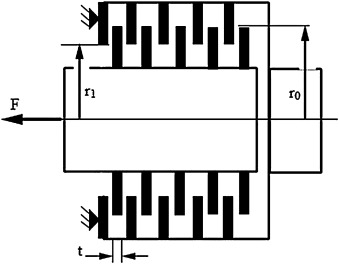
\includegraphics[scale=0.6]{Imgs/MD.jpg}
    \end{center}
    \captionsetup{justification=centering}
    \caption{Schematic view of the multiple disk clutch brake design problem.}\label{fig:MD}
\end{figure}


\prob{Appendix/Problems/MD}